\chapter{Introduction}
\label{ch:intro}

\section{Background}
\label{s:background}

The notion of describing amorphous materials as random networks dates back to \zach, who in 1932 sketched a simple diagram of a \td{} glass \cite{Zachariasen1932}.
This configuration, reproduced in figure \ref{fig:zach_orig}, showed a collection of percolating rings with an absence of long\--range order.
At the time, \zach's image was intended only as schematic to illustrate the analogous effects in \thd{} glasses.
However, some eighty years later, modern synthesis techniques have led to a range of \td{} materials including amorphous carbon, silica and germania which can be considered realisations of \zach's glass \cite{Kotakoski2011,Robertson2012,Huang2012,Lichtenstein2012b,Lewandowski2018}.
These advances may yet represent a watershed moment in chemistry, facilitating the development of a wide range of technologically useful materials with applications including catalysis and gas separation \cite{Trogadas2014,Sun2015a,Buchner2017}.

It is clear that understanding the structure of amorphous materials is key to this aim.
However, due to the relative recentness of these experimental discoveries, much of the existing theory arises from studies of systems on greater length scales.
Specifically, in the second half of the 20\th{} century, much work was done on the formation of polycrystals in metals and alloys .
By annealing the metal and slicing through the sample, the grains in the polycrystal could be directly imaged; revealing a system of tessellating polygons not dissimilar to an atomic material \cite{Beck1954,Dunn1957}.
Over time it became apparent that the structure of these networks is constrained on a series of different levels.

Firstly the mean ring size (\ie{} the average number of sides in a polygon) tends to the constant value of six.
This is readily explainable via graph theoretic arguments, simply resulting from Euler's formula when each vertex forms part of three edges - as is the case for trivalent atoms or the meeting of three grain boundaries.
Intuitively from chemistry we know this to be true: a pristine graphene sheet is a hexagonal net and although a Stone\--Wales defect introduces pentagons and heptagons, they occur in pairs to preserve the overall mean ring size \cite{Stone1986}.

The next level of information is then the explicit distribution of polygon sizes, also known as the ring statistics.
With the constraint of a fixed mean, the ring statistics were shown to be relatively well defined, following a log\--normal or maximum entropy distribution \cite{Shackelford1981,Lemaitre1993,Lichtenstein2012}.
However, the ring statistics alone are not sufficient to fully describe the network topology. 
This is because the same set of rings can be arranged in a large number of different ways.
Consider again \zach's original configuration. 
Removing one square achieves a mean ring size of six and allows the constituent rings to be arranged as a periodic tiling.
Figures \ref{fig:zach_high}\--\ref{fig:zach_low} show three such examples tilings.


\begin{figure}[h]
     \centering
     
     \begin{subfigure}[b]{0.25\textwidth}
         \centering
         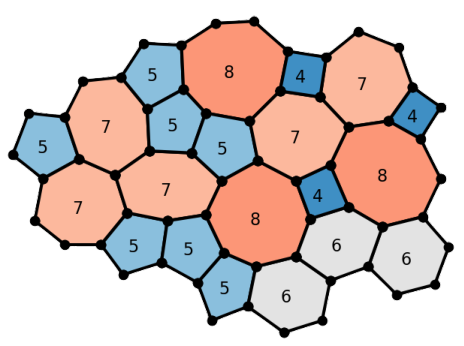
\includegraphics[width=\textwidth]{./figures/introduction/zach_orig.pdf}
         \caption{}
         \label{fig:zach_orig}
     \end{subfigure}
     \hspace{1cm}
     \begin{subfigure}[b]{0.25\textwidth}
         \centering
         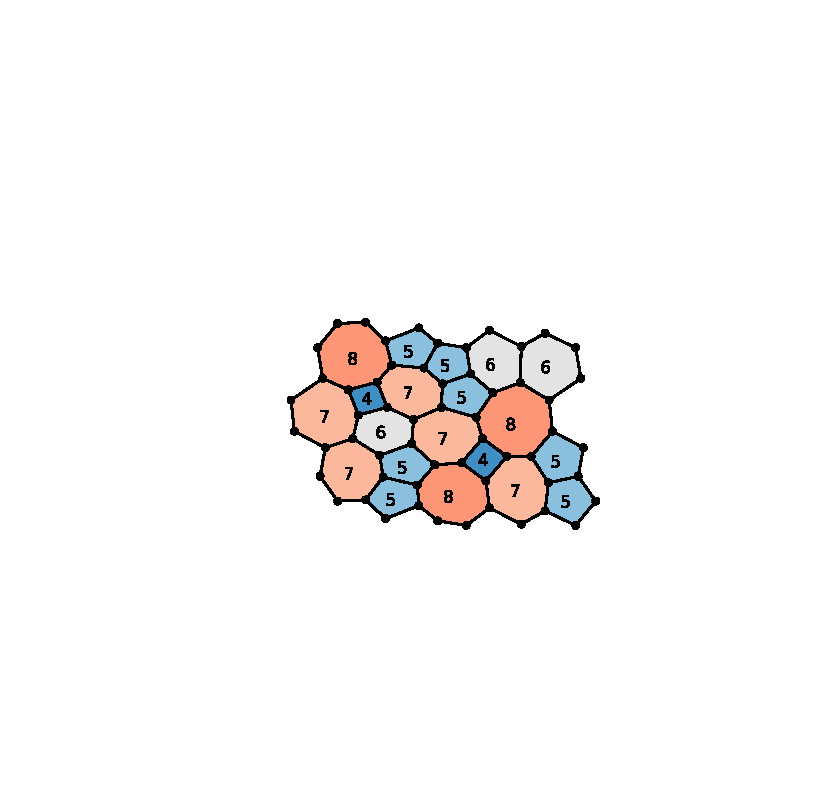
\includegraphics[width=\textwidth]{./figures/introduction/zach_high.pdf}
         \caption{}
         \label{fig:zach_high}
     \end{subfigure}
     \hspace{1cm}
     
     \begin{subfigure}[b]{0.25\textwidth}
         \centering
         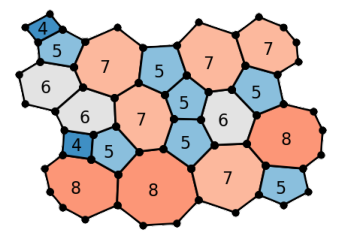
\includegraphics[width=\textwidth]{./figures/introduction/zach_mid.pdf}
         \caption{}
     \end{subfigure}
     \hspace{1cm}
     \begin{subfigure}[b]{0.25\textwidth}
         \centering
         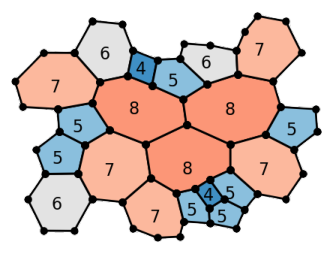
\includegraphics[width=\textwidth]{./figures/introduction/zach_low.pdf}
         \caption{}
         \label{fig:zach_low}
     \end{subfigure}
     
     \caption{Panel (a) shows \zach's glass and panels (b)\--(d) three different periodic arrangements based on the glass (with one square removed to satisfy Euler's formula). Moving from panel (b)\--(d) there is increased clustering of similar sized rings. The size of the rings are highlighted numerically and by colour.}
     \label{fig:zach}
\end{figure}

Whilst they may initially look similar, on closer inspection the three configurations display fundamentally different properties.
In figure \ref{fig:zach_high} similar sized rings are dispersed throughout the arrangement whilst in \ref{fig:zach_low} they are tightly clustered together.
Furthermore, given the large number of configurations which may be theoretically possible for any set of ring statistics, only a subset of these may be physically realisable.
Empirically, these are found to be the ones in which large rings tend to be surrounded by smaller rings \ie{} similar to \ref{fig:zach_high}.
Once again, chemical intuition would support this in the context of atomic materials, as strain is minimised by maintaining bond lengths and angles as close to their equilibrium values as possible.

This effect was first noticed in polycrystals and quantified through the \aw{} law \cite{Aboav1970,Weaire1974}.
This law claims that the mean ring size about any given ring can be related to the central ring size by a single fitting parameter.
Hence the value of this parameter in some way describes the increased tendency of the small rings to be adjacent to large rings in a network.
Perhaps surprisingly, this law holds for a wide range of physical systems, originally encompassing metal oxides, foams and Voronoi polygons \cite{Aboav1980,Boots1984}.

It is now clear that these chemical networks fit into a much wider class of \td{} physical networks that are ubiquitous in the natural world, emerging across all physical disciplines and length scales.
Traditional examples range from the atomic level of ultra\--thin materials, through colloids, foams, epithelial cells and all the way to geological rock formations \cite{Earnshaw1994,Allain1995,Durand2011,Tong2017,Goehring2014}.
There are however countless more occurrences, with drying blood, stratocumulus clouds, crocodile scales and geopolitical borders all being the subject of studies \cite{Brutin2011,Glassmeier2017,Milinkovitch2019,LeCaer1993}.
More intriguingly, although these systems are incredibly physically diverse, they still have similar structures \cite{Schliecker1999}. 
This is because they can all be mapped onto the same generic system, which can be equivalently described as a collection of tessellating polygons or percolating rings, and hence they are governed by the same fundamental laws. 

Understanding the behaviours of \td{} networks is therefore key to a wide range of problems in frontier research, not only the directed synthesis of nano\--materials but also for example the control of mitotic division \cite{Malashevich2016,Gibson2011,Ladan2019}; as well as to curiosities such as explaining the arrangement of the stones in Giant's Causeway or cracking in famous artwork \cite{Weaire1984,Flores2017}.


 



\section{Thesis Structure}


